% author Truong Nhan Nguyen

\documentclass[tikz, border=10pt]{standalone}

\usepackage{amsmath, amsfonts, amssymb, mathtools}
\usepackage{graphics}
\usepackage{xcolor}
% define colors
\definecolor{mediumpurple}{RGB}{147,112,219}
\definecolor{telemagenta}{RGB}{207,52,118}
\definecolor{crimson}{RGB}{220,20,60}
\definecolor{darkorange}{RGB}{255,140,0}
\definecolor{gold}{RGB}{255,215,0}
\usepackage{tikz}
% define styles
\tikzset{
    node/.style = {draw=white, fill=black!50, circle, minimum size=20pt},
    inp/.style = {node, fill=mediumpurple},
    hl1/.style = {node, fill=telemagenta},
    hl2/.style = {node, fill=crimson},
    hl3/.style = {node, fill=darkorange},
    op/.style = {node, fill=gold}
}

\begin{document}
    \begin{tikzpicture}
        \bfseries\sffamily
        % draw layers
        \foreach \y in {0, 1, 2, 3, 4, 5}{
            % Input layer
            \node[inp] (inp-\y) at (0, \y) {};
            % Hidden layer 1
            \node[hl1] (hl1-\y) at (3, \y) {};
            % Hidden layer 2
            \node[hl2] (hl2-\y) at (6, \y) {};
            % Hidden layer 3
            \node[hl3] (hl3-\y) at (9, \y) {};
        }
        \foreach \y in {2, 3}{
            % Output layer
            \node[op, pin={[pin edge={-latex, gold}, pin distance=1.5cm]right:$ $}] (op-\y) at (12, \y) {};
        }
        % draw connecting lines
        \foreach \x in {0, 1, 2, 3, 4, 5}{
            \foreach \y in {0, 1, 2, 3, 4, 5}{
                % from input layer to hidden layer 1
                \draw[mediumpurple] (inp-\x) -- (hl1-\y);
                % from hidden layer 1 to hidden layer 2
                \draw[telemagenta] (hl1-\x) -- (hl2-\y);
                % from hidden layer 2 to hidden layer 3
                \draw[crimson] (hl2-\x) -- (hl3-\y);
            }
        }
        % from hidden layer 3 to output layer
        \foreach \x in {0, 1, 2, 3, 4, 5}{
            \foreach \y in {2, 3}{
                \draw[darkorange] (hl3-\x) -- (op-\y);
            }
        }
        % from source to input layer
        \foreach \x in {0, 1, 2}{
            \draw[dashed, -latex, mediumpurple] (-1, 2.5) to[out=-60, in=180] (inp-\x);
        }
        \foreach \x in {3, 4, 5}{
            \draw[dashed, -latex, mediumpurple] (-1, 2.5) to[out=60, in=180] (inp-\x);
        }
        % add names of label, feature/image, input layer, hidden layer and output layer
        \foreach \pos/\layer/\label/\name/\col in {
            inp-5/T_0=X/inp/(Input Layer)/mediumpurple,
            hl1-5/T_1/hl1/(Hidden Layer 1)/telemagenta,
            hl2-5/T_2/hl2/(Hidden Layer 2)/crimson,
            hl3-5/T_3/hl3/(Hidden Layer 3)/darkorange%
        }{
            \node[anchor=south, text width=3cm, text centered, inner sep=0pt] (\label) at (\pos.north) {\color{\col}$\mathsf{\layer}$ \\[-2pt] \name};
        }
        \node[anchor=south, text width=2cm, text centered, inner sep=0pt, yshift=0.75cm] at (op-3.north) {$\mathsf{\textcolor{gold}{T_4}=\textcolor{green}{\widehat{Y}}}$ \\[-2pt] \textcolor{gold}{Output Layer}};
        \node[text width=2cm, text centered, inner sep=0pt, xshift=-1.75cm, color=blue!50] (feature/image) [left of=inp] {$\mathsf{X}$ \\[-2pt] Feature/Image};
        \node[text width=2cm, text centered, inner sep=0pt, xshift=-1.5cm, color=green] (label) [left of=feature/image] {$\mathsf{Y}$ \\[-2pt] Label};
        % add names of image
        \node[below of = label, yshift=-1.25cm, color=green] {Cat};
        \node[below of = label, yshift=-3cm, color=green] {Dog};
        % add images
        \node[below of = feature/image, yshift=-1.25cm, xshift=0.2cm] {
\includegraphics[scale=0.05]{./images/cat.jpg}};
        \node[below of = feature/image, yshift=-3cm, xshift=0.2cm] {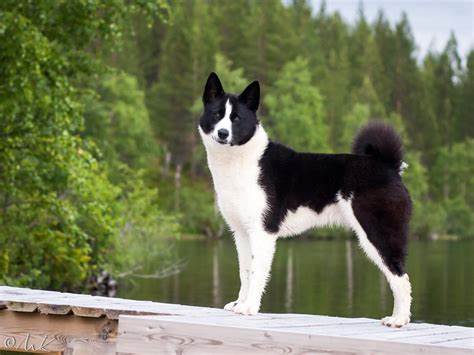
\includegraphics[scale=0.135]{./images/dog.jpg}};
    \end{tikzpicture}
\end{document}